% Options for packages loaded elsewhere
\PassOptionsToPackage{unicode}{hyperref}
\PassOptionsToPackage{hyphens}{url}
\PassOptionsToPackage{dvipsnames,svgnames,x11names}{xcolor}
%
\documentclass[
  letterpaper,
  DIV=11,
  numbers=noendperiod,
  oneside]{scrartcl}

\usepackage{amsmath,amssymb}
\usepackage{lmodern}
\usepackage{iftex}
\ifPDFTeX
  \usepackage[T1]{fontenc}
  \usepackage[utf8]{inputenc}
  \usepackage{textcomp} % provide euro and other symbols
\else % if luatex or xetex
  \usepackage{unicode-math}
  \defaultfontfeatures{Scale=MatchLowercase}
  \defaultfontfeatures[\rmfamily]{Ligatures=TeX,Scale=1}
\fi
% Use upquote if available, for straight quotes in verbatim environments
\IfFileExists{upquote.sty}{\usepackage{upquote}}{}
\IfFileExists{microtype.sty}{% use microtype if available
  \usepackage[]{microtype}
  \UseMicrotypeSet[protrusion]{basicmath} % disable protrusion for tt fonts
}{}
\makeatletter
\@ifundefined{KOMAClassName}{% if non-KOMA class
  \IfFileExists{parskip.sty}{%
    \usepackage{parskip}
  }{% else
    \setlength{\parindent}{0pt}
    \setlength{\parskip}{6pt plus 2pt minus 1pt}}
}{% if KOMA class
  \KOMAoptions{parskip=half}}
\makeatother
\usepackage{xcolor}
\usepackage[left=1in,marginparwidth=2.0666666666667in,textwidth=4.1333333333333in,marginparsep=0.3in]{geometry}
\setlength{\emergencystretch}{3em} % prevent overfull lines
\setcounter{secnumdepth}{-\maxdimen} % remove section numbering
% Make \paragraph and \subparagraph free-standing
\ifx\paragraph\undefined\else
  \let\oldparagraph\paragraph
  \renewcommand{\paragraph}[1]{\oldparagraph{#1}\mbox{}}
\fi
\ifx\subparagraph\undefined\else
  \let\oldsubparagraph\subparagraph
  \renewcommand{\subparagraph}[1]{\oldsubparagraph{#1}\mbox{}}
\fi

\usepackage{color}
\usepackage{fancyvrb}
\newcommand{\VerbBar}{|}
\newcommand{\VERB}{\Verb[commandchars=\\\{\}]}
\DefineVerbatimEnvironment{Highlighting}{Verbatim}{commandchars=\\\{\}}
% Add ',fontsize=\small' for more characters per line
\usepackage{framed}
\definecolor{shadecolor}{RGB}{241,243,245}
\newenvironment{Shaded}{\begin{snugshade}}{\end{snugshade}}
\newcommand{\AlertTok}[1]{\textcolor[rgb]{0.68,0.00,0.00}{#1}}
\newcommand{\AnnotationTok}[1]{\textcolor[rgb]{0.37,0.37,0.37}{#1}}
\newcommand{\AttributeTok}[1]{\textcolor[rgb]{0.40,0.45,0.13}{#1}}
\newcommand{\BaseNTok}[1]{\textcolor[rgb]{0.68,0.00,0.00}{#1}}
\newcommand{\BuiltInTok}[1]{\textcolor[rgb]{0.00,0.23,0.31}{#1}}
\newcommand{\CharTok}[1]{\textcolor[rgb]{0.13,0.47,0.30}{#1}}
\newcommand{\CommentTok}[1]{\textcolor[rgb]{0.37,0.37,0.37}{#1}}
\newcommand{\CommentVarTok}[1]{\textcolor[rgb]{0.37,0.37,0.37}{\textit{#1}}}
\newcommand{\ConstantTok}[1]{\textcolor[rgb]{0.56,0.35,0.01}{#1}}
\newcommand{\ControlFlowTok}[1]{\textcolor[rgb]{0.00,0.23,0.31}{#1}}
\newcommand{\DataTypeTok}[1]{\textcolor[rgb]{0.68,0.00,0.00}{#1}}
\newcommand{\DecValTok}[1]{\textcolor[rgb]{0.68,0.00,0.00}{#1}}
\newcommand{\DocumentationTok}[1]{\textcolor[rgb]{0.37,0.37,0.37}{\textit{#1}}}
\newcommand{\ErrorTok}[1]{\textcolor[rgb]{0.68,0.00,0.00}{#1}}
\newcommand{\ExtensionTok}[1]{\textcolor[rgb]{0.00,0.23,0.31}{#1}}
\newcommand{\FloatTok}[1]{\textcolor[rgb]{0.68,0.00,0.00}{#1}}
\newcommand{\FunctionTok}[1]{\textcolor[rgb]{0.28,0.35,0.67}{#1}}
\newcommand{\ImportTok}[1]{\textcolor[rgb]{0.00,0.46,0.62}{#1}}
\newcommand{\InformationTok}[1]{\textcolor[rgb]{0.37,0.37,0.37}{#1}}
\newcommand{\KeywordTok}[1]{\textcolor[rgb]{0.00,0.23,0.31}{#1}}
\newcommand{\NormalTok}[1]{\textcolor[rgb]{0.00,0.23,0.31}{#1}}
\newcommand{\OperatorTok}[1]{\textcolor[rgb]{0.37,0.37,0.37}{#1}}
\newcommand{\OtherTok}[1]{\textcolor[rgb]{0.00,0.23,0.31}{#1}}
\newcommand{\PreprocessorTok}[1]{\textcolor[rgb]{0.68,0.00,0.00}{#1}}
\newcommand{\RegionMarkerTok}[1]{\textcolor[rgb]{0.00,0.23,0.31}{#1}}
\newcommand{\SpecialCharTok}[1]{\textcolor[rgb]{0.37,0.37,0.37}{#1}}
\newcommand{\SpecialStringTok}[1]{\textcolor[rgb]{0.13,0.47,0.30}{#1}}
\newcommand{\StringTok}[1]{\textcolor[rgb]{0.13,0.47,0.30}{#1}}
\newcommand{\VariableTok}[1]{\textcolor[rgb]{0.07,0.07,0.07}{#1}}
\newcommand{\VerbatimStringTok}[1]{\textcolor[rgb]{0.13,0.47,0.30}{#1}}
\newcommand{\WarningTok}[1]{\textcolor[rgb]{0.37,0.37,0.37}{\textit{#1}}}

\providecommand{\tightlist}{%
  \setlength{\itemsep}{0pt}\setlength{\parskip}{0pt}}\usepackage{longtable,booktabs,array}
\usepackage{calc} % for calculating minipage widths
% Correct order of tables after \paragraph or \subparagraph
\usepackage{etoolbox}
\makeatletter
\patchcmd\longtable{\par}{\if@noskipsec\mbox{}\fi\par}{}{}
\makeatother
% Allow footnotes in longtable head/foot
\IfFileExists{footnotehyper.sty}{\usepackage{footnotehyper}}{\usepackage{footnote}}
\makesavenoteenv{longtable}
\usepackage{graphicx}
\makeatletter
\def\maxwidth{\ifdim\Gin@nat@width>\linewidth\linewidth\else\Gin@nat@width\fi}
\def\maxheight{\ifdim\Gin@nat@height>\textheight\textheight\else\Gin@nat@height\fi}
\makeatother
% Scale images if necessary, so that they will not overflow the page
% margins by default, and it is still possible to overwrite the defaults
% using explicit options in \includegraphics[width, height, ...]{}
\setkeys{Gin}{width=\maxwidth,height=\maxheight,keepaspectratio}
% Set default figure placement to htbp
\makeatletter
\def\fps@figure{htbp}
\makeatother

\KOMAoption{captions}{tableheading}
\makeatletter
\@ifpackageloaded{tcolorbox}{}{\usepackage[many]{tcolorbox}}
\@ifpackageloaded{fontawesome5}{}{\usepackage{fontawesome5}}
\definecolor{quarto-callout-color}{HTML}{909090}
\definecolor{quarto-callout-note-color}{HTML}{0758E5}
\definecolor{quarto-callout-important-color}{HTML}{CC1914}
\definecolor{quarto-callout-warning-color}{HTML}{EB9113}
\definecolor{quarto-callout-tip-color}{HTML}{00A047}
\definecolor{quarto-callout-caution-color}{HTML}{FC5300}
\definecolor{quarto-callout-color-frame}{HTML}{acacac}
\definecolor{quarto-callout-note-color-frame}{HTML}{4582ec}
\definecolor{quarto-callout-important-color-frame}{HTML}{d9534f}
\definecolor{quarto-callout-warning-color-frame}{HTML}{f0ad4e}
\definecolor{quarto-callout-tip-color-frame}{HTML}{02b875}
\definecolor{quarto-callout-caution-color-frame}{HTML}{fd7e14}
\makeatother
\makeatletter
\makeatother
\makeatletter
\makeatother
\makeatletter
\@ifpackageloaded{caption}{}{\usepackage{caption}}
\AtBeginDocument{%
\ifdefined\contentsname
  \renewcommand*\contentsname{Table of contents}
\else
  \newcommand\contentsname{Table of contents}
\fi
\ifdefined\listfigurename
  \renewcommand*\listfigurename{List of Figures}
\else
  \newcommand\listfigurename{List of Figures}
\fi
\ifdefined\listtablename
  \renewcommand*\listtablename{List of Tables}
\else
  \newcommand\listtablename{List of Tables}
\fi
\ifdefined\figurename
  \renewcommand*\figurename{Figure}
\else
  \newcommand\figurename{Figure}
\fi
\ifdefined\tablename
  \renewcommand*\tablename{Table}
\else
  \newcommand\tablename{Table}
\fi
}
\@ifpackageloaded{float}{}{\usepackage{float}}
\floatstyle{ruled}
\@ifundefined{c@chapter}{\newfloat{codelisting}{h}{lop}}{\newfloat{codelisting}{h}{lop}[chapter]}
\floatname{codelisting}{Listing}
\newcommand*\listoflistings{\listof{codelisting}{List of Listings}}
\makeatother
\makeatletter
\@ifpackageloaded{caption}{}{\usepackage{caption}}
\@ifpackageloaded{subcaption}{}{\usepackage{subcaption}}
\makeatother
\makeatletter
\@ifpackageloaded{tcolorbox}{}{\usepackage[many]{tcolorbox}}
\makeatother
\makeatletter
\@ifundefined{shadecolor}{\definecolor{shadecolor}{rgb}{.97, .97, .97}}
\makeatother
\makeatletter
\@ifpackageloaded{sidenotes}{}{\usepackage{sidenotes}}
\@ifpackageloaded{marginnote}{}{\usepackage{marginnote}}
\makeatother
\makeatletter
\makeatother
\ifLuaTeX
  \usepackage{selnolig}  % disable illegal ligatures
\fi
\IfFileExists{bookmark.sty}{\usepackage{bookmark}}{\usepackage{hyperref}}
\IfFileExists{xurl.sty}{\usepackage{xurl}}{} % add URL line breaks if available
\urlstyle{same} % disable monospaced font for URLs
\hypersetup{
  colorlinks=true,
  linkcolor={blue},
  filecolor={Maroon},
  citecolor={Blue},
  urlcolor={Blue},
  pdfcreator={LaTeX via pandoc}}

\author{}
\date{}

\begin{document}
\ifdefined\Shaded\renewenvironment{Shaded}{\begin{tcolorbox}[frame hidden, breakable, interior hidden, enhanced, borderline west={3pt}{0pt}{shadecolor}, sharp corners, boxrule=0pt]}{\end{tcolorbox}}\fi

\hypertarget{introduction}{%
\section{Introduction}\label{introduction}}

This document demonstrates the use of a number of these page layout
features to produce an attractive and usable document inspired by the
Tufte handout style and the use of Tufte's styles in RMarkdown documents
{[}@xie2018{]}. The Tufte handout style is a style that Edward Tufte
uses in his books and handouts. Tufte's style is known for its extensive
use of sidenotes, tight integration of graphics with text, and well-set
typography. Quarto\footnote{To learn more, you can read more about
  \href{https://www.quarto.org}{Quarto} or visit
  \href{https://www.github.com/quarto-dev/quarto-cli}{Quarto's Github
  repository}.} supports most of the layout techniques that are used in
the Tufte handout style for both HTML and LaTeX/PDF output.

\begin{Shaded}
\begin{Highlighting}[]
\PreprocessorTok{{-}{-}{-}}
\FunctionTok{title}\KeywordTok{:}\AttributeTok{ }\StringTok{"An Example Using the Tufte Style"}
\FunctionTok{author}\KeywordTok{:}\AttributeTok{ }\StringTok{"John Smith"}
\FunctionTok{format}\KeywordTok{:}
\AttributeTok{  }\FunctionTok{html}\KeywordTok{:}\AttributeTok{ default}
\AttributeTok{  }\FunctionTok{pdf}\KeywordTok{:}\AttributeTok{ default}
\AttributeTok{  }
\CommentTok{\# places footnotes and cited sources in the margin}
\CommentTok{\# other layout options (for example placing a }
\CommentTok{\# figure in the margin)  will be set on per element}
\CommentTok{\# in examples below}
\FunctionTok{reference{-}location}\KeywordTok{:}\AttributeTok{ margin}
\PreprocessorTok{{-}{-}{-}}
\end{Highlighting}
\end{Shaded}

These layout features are designed with two important goals in mind:

\begin{enumerate}
\def\labelenumi{\arabic{enumi}.}
\tightlist
\item
  To produce both PDF and HTML output with similar styles from the same
  Quarto document;
\item
  To provide simple syntax to write elements of the Tufte style such as
  side notes and margin figures. If you'd like a figure placed in the
  margin, just set the option \texttt{fig-column:\ margin} for your code
  chunk, and we will take care of the details for you\footnote{You never
    need to think about \texttt{\textbackslash{}begin\{marginfigure\}}
    or \texttt{\textless{}span\ class="marginfigure"\textgreater{}}; the
    LaTeX and HTML code under the hood may be complicated, but you never
    need to learn or write such code.}.
\end{enumerate}

If you have any feature requests or find bugs in this capabilities,
please do not hesitate to file them to
\href{https://github.com/rstudio/tufte/issues}{https://github.com/quarto-dev/quarto-cli/issues}.

\hypertarget{figures}{%
\section{Figures}\label{figures}}

\hypertarget{margin-figures}{%
\subsection{Margin Figures}\label{margin-figures}}

Images and graphics play an integral role in Tufte's work. To place
figures in the margin you can use the \textbf{Quarto} chunk option
\texttt{column:\ margin}. For example:

\begin{Shaded}
\begin{Highlighting}[]
\FunctionTok{library}\NormalTok{(ggplot2)}
\NormalTok{mtcars2 }\OtherTok{\textless{}{-}}\NormalTok{ mtcars}
\NormalTok{mtcars2}\SpecialCharTok{$}\NormalTok{am }\OtherTok{\textless{}{-}} \FunctionTok{factor}\NormalTok{(}
\NormalTok{  mtcars}\SpecialCharTok{$}\NormalTok{am, }\AttributeTok{labels =} \FunctionTok{c}\NormalTok{(}\StringTok{\textquotesingle{}automatic\textquotesingle{}}\NormalTok{, }\StringTok{\textquotesingle{}manual\textquotesingle{}}\NormalTok{)}
\NormalTok{)}
\FunctionTok{ggplot}\NormalTok{(mtcars2, }\FunctionTok{aes}\NormalTok{(hp, mpg, }\AttributeTok{color =}\NormalTok{ am)) }\SpecialCharTok{+}
  \FunctionTok{geom\_point}\NormalTok{() }\SpecialCharTok{+} \FunctionTok{geom\_smooth}\NormalTok{() }\SpecialCharTok{+}
  \FunctionTok{theme}\NormalTok{(}\AttributeTok{legend.position =} \StringTok{\textquotesingle{}bottom\textquotesingle{}}\NormalTok{)}
\end{Highlighting}
\end{Shaded}

\begin{marginfigure}

{\centering 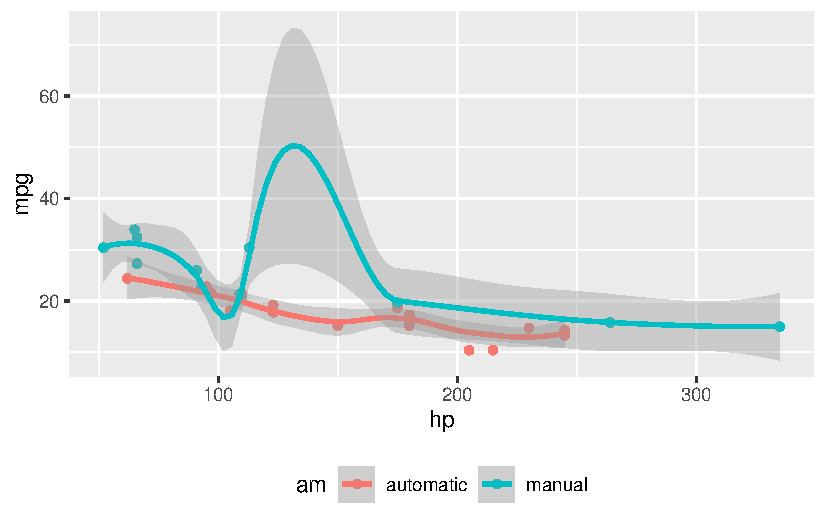
\includegraphics{cv_files/figure-pdf/fig-margin-1.pdf}

}

\caption{\label{fig-margin}MPG vs horsepower, colored by transmission.}

\end{marginfigure}

Note the use of the \texttt{fig-cap} chunk option to provide a figure
caption. You can adjust the proportions of figures using the
\texttt{fig-width} and \texttt{fig-height} chunk options. These are
specified in inches, and will be automatically scaled down to fit within
the handout margin.

\hypertarget{arbitrary-margin-content}{%
\subsection{Arbitrary Margin Content}\label{arbitrary-margin-content}}

You can include anything in the margin by places the class
\texttt{.column-margin} on the element. See an example on the right
about the first fundamental theorem of calculus.

\marginnote{\begin{footnotesize}

We know from \emph{the first fundamental theorem of calculus} that for
\(x\) in \([a, b]\):

\[\frac{d}{dx}\left( \int_{a}^{x} f(u)\,du\right)=f(x).\]

\end{footnotesize}}

\hypertarget{full-width-figures}{%
\subsection{Full Width Figures}\label{full-width-figures}}

You can arrange for figures to span across the entire page by using the
chunk option \texttt{fig-column:\ page-right}.

\begin{Shaded}
\begin{Highlighting}[]
\FunctionTok{ggplot}\NormalTok{(diamonds, }\FunctionTok{aes}\NormalTok{(carat, price)) }\SpecialCharTok{+} \FunctionTok{geom\_smooth}\NormalTok{() }\SpecialCharTok{+}
  \FunctionTok{facet\_grid}\NormalTok{(}\SpecialCharTok{\textasciitilde{}}\NormalTok{ cut)}
\end{Highlighting}
\end{Shaded}

\begin{figure*}[H]

{\centering 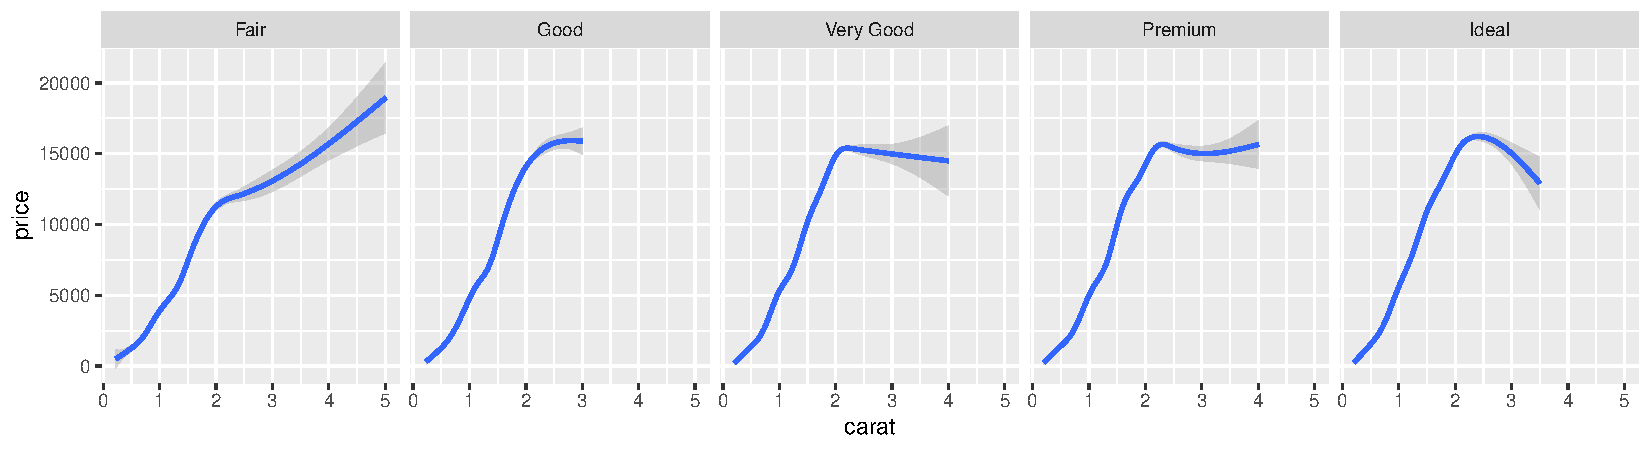
\includegraphics{cv_files/figure-pdf/fig-fullwidth-1.pdf}

}

\caption{\label{fig-fullwidth}A full width figure.}

\end{figure*}

Other chunk options related to figures can still be used, such as
\texttt{fig-width}, \texttt{fig-cap}, and so on. For full width figures,
usually \texttt{fig-width} is large and \texttt{fig-height} is small. In
the above example, the plot size is \(11 \times 3\).

\hypertarget{arbitrary-full-width-content}{%
\subsection{Arbitrary Full Width
Content}\label{arbitrary-full-width-content}}

Any content can span to the full width of the page, simply place the
element in a \texttt{div} and add the class \texttt{column-page-right}.
For example, the following code will display its contents as full width.

\begin{Shaded}
\begin{Highlighting}[]
\NormalTok{::: \{.fullwidth\}}
\NormalTok{Any \_full width\_ content here.}
\NormalTok{:::}
\end{Highlighting}
\end{Shaded}

Below is an example:

\begin{figure*}

\emph{R is free software and comes with ABSOLUTELY NO WARRANTY.} You are
welcome to redistribute it under the terms of the GNU General Public
License versions 2 or 3. For more information about these matters see
https://www.gnu.org/licenses/.

\end{figure*}

\hypertarget{main-column-figures}{%
\subsection{Main Column Figures}\label{main-column-figures}}

Besides margin and full width figures, you can of course also include
figures constrained to the main column. This is the default type of
figures in the LaTeX/HTML output.

\begin{Shaded}
\begin{Highlighting}[]
\FunctionTok{ggplot}\NormalTok{(diamonds, }\FunctionTok{aes}\NormalTok{(cut, price)) }\SpecialCharTok{+} \FunctionTok{geom\_boxplot}\NormalTok{()}
\end{Highlighting}
\end{Shaded}

\begin{figure}[H]

{\centering 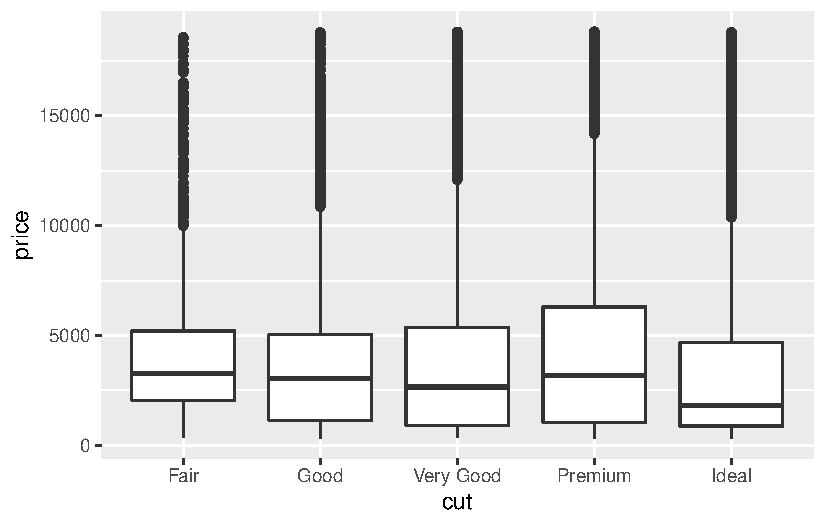
\includegraphics{cv_files/figure-pdf/fig-main-1.pdf}

}

\caption{\label{fig-main}A figure in the main column.}

\end{figure}

\hypertarget{margin-captions}{%
\subsection{Margin Captions}\label{margin-captions}}

When you include a figure constrained to the main column, you can choose
to place the figure's caption in the margin by using the
\texttt{cap-location} chunk option. For example:

\begin{Shaded}
\begin{Highlighting}[]
\FunctionTok{ggplot}\NormalTok{(diamonds, }\FunctionTok{aes}\NormalTok{(cut, price)) }\SpecialCharTok{+} \FunctionTok{geom\_boxplot}\NormalTok{()}
\end{Highlighting}
\end{Shaded}

\begin{figure}[H]

\sidecaption{\label{fig-main-margin-cap}A figure with a longer caption.
The figure appears in the main column, but the caption is placed in the
margin. Caption can even contain elements like a citation such as
@xie2018.}

{\centering 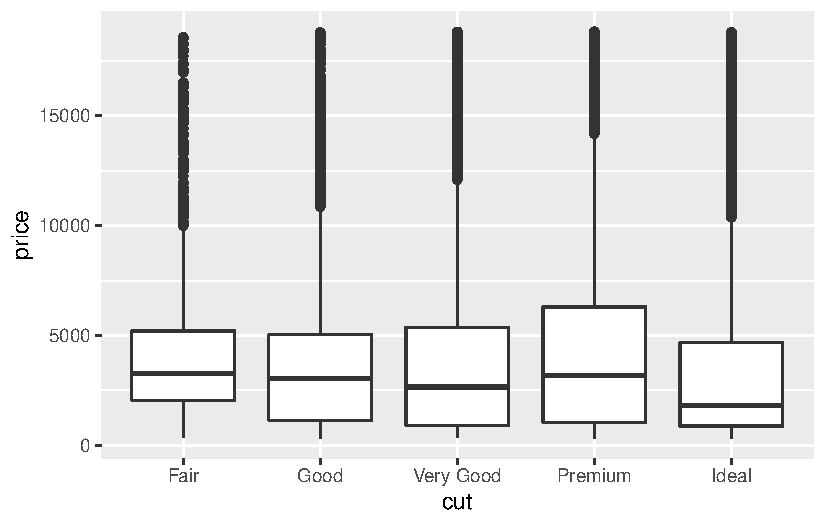
\includegraphics{cv_files/figure-pdf/fig-main-margin-cap-1.pdf}

}

\end{figure}

\hypertarget{sidenotes}{%
\section{Sidenotes}\label{sidenotes}}

One of the most prominent and distinctive features of this style is the
extensive use of sidenotes. There is a wide margin to provide ample room
for sidenotes and small figures. Any use of a footnote will
automatically be converted to a sidenote.

{\marginnote{\begin{footnotesize}This is a span that has the class
\texttt{column-margin} which places it in the margin without the
sidenote mark.\end{footnotesize}}} If you'd like to place ancillary
information in the margin without the sidenote mark (the superscript
number), you can use apply the \texttt{column-margin} class to the
element.

\hypertarget{references}{%
\section{References}\label{references}}

References can be displayed as margin notes for HTML output. For
example, we can cite R here {[}@R-base{]}.

\begin{tcolorbox}[enhanced jigsaw, left=2mm, bottomrule=.15mm, colframe=quarto-callout-note-color-frame, opacityback=0, leftrule=.75mm, rightrule=.15mm, breakable, toprule=.15mm, arc=.35mm, colback=white]
\begin{minipage}[t]{5.5mm}
\textcolor{quarto-callout-note-color}{\faInfo}
\end{minipage}%
\begin{minipage}[t]{\textwidth - 5.5mm}
This feature depends upon \texttt{link-citations} to locate and place
references in the margin. This is enabled by default, but if you disable
\texttt{link-citations} then references in the HTML output will be
placed at the end of the output document as they normally
are.\end{minipage}%
\end{tcolorbox}

\hypertarget{tables}{%
\section{Tables}\label{tables}}

You can use the \texttt{kable()} function from the \textbf{knitr}
package to format tables that integrate well with the rest of the Tufte
handout style. The table captions are placed in the margin like figures
in the HTML output.

\begin{Shaded}
\begin{Highlighting}[]
\NormalTok{knitr}\SpecialCharTok{::}\FunctionTok{kable}\NormalTok{(}
\NormalTok{  mtcars[}\DecValTok{1}\SpecialCharTok{:}\DecValTok{6}\NormalTok{, }\DecValTok{1}\SpecialCharTok{:}\DecValTok{6}\NormalTok{], }\AttributeTok{caption =} \StringTok{\textquotesingle{}A subset of mtcars.\textquotesingle{}}
\NormalTok{)}
\end{Highlighting}
\end{Shaded}

{
\makeatletter
\def\LT@makecaption#1#2#3{%
  \noalign{\smash{\hbox{\kern\textwidth\rlap{\kern\marginparsep
  \parbox[t]{\marginparwidth}{%
    \footnotesize{%
      \vspace{(1.1\baselineskip)}
    #1{#2: }\ignorespaces #3}}}}}}%
    }
\makeatother

\begin{longtable}[]{@{}lrrrrrr@{}}
\caption{A subset of mtcars.}\tabularnewline
\toprule()
& mpg & cyl & disp & hp & drat & wt \\
\midrule()
\endfirsthead
\toprule()
& mpg & cyl & disp & hp & drat & wt \\
\midrule()
\endhead
Mazda RX4 & 21.0 & 6 & 160 & 110 & 3.90 & 2.620 \\
Mazda RX4 Wag & 21.0 & 6 & 160 & 110 & 3.90 & 2.875 \\
Datsun 710 & 22.8 & 4 & 108 & 93 & 3.85 & 2.320 \\
Hornet 4 Drive & 21.4 & 6 & 258 & 110 & 3.08 & 3.215 \\
Hornet Sportabout & 18.7 & 8 & 360 & 175 & 3.15 & 3.440 \\
Valiant & 18.1 & 6 & 225 & 105 & 2.76 & 3.460 \\
\bottomrule()
\end{longtable}

}

\hypertarget{responsiveness}{%
\section{Responsiveness}\label{responsiveness}}

The HTML page layout is responsive- as the page width shrinks, elements
will automatically adjust their position. Elements that appear in the
margins will move inline with the content and elements that span the
body and margin will automatically span only the body.

\hypertarget{more-examples}{%
\section{More Examples}\label{more-examples}}

The rest of this document consists of a few test cases to make sure
everything still works well in slightly more complicated scenarios.
First we generate two plots in one figure environment with the chunk
option \texttt{fig.show\ =\ \textquotesingle{}hold\textquotesingle{}}:

\begin{Shaded}
\begin{Highlighting}[]
\NormalTok{p }\OtherTok{\textless{}{-}} \FunctionTok{ggplot}\NormalTok{(mtcars2, }\FunctionTok{aes}\NormalTok{(hp, mpg, }\AttributeTok{color =}\NormalTok{ am)) }\SpecialCharTok{+}
  \FunctionTok{geom\_point}\NormalTok{()}
\NormalTok{p}
\NormalTok{p }\SpecialCharTok{+} \FunctionTok{geom\_smooth}\NormalTok{()}
\end{Highlighting}
\end{Shaded}

\begin{figure}[H]

\sidecaption{\label{fig-two-together-1}Two plots in one figure
environment.}

{\centering 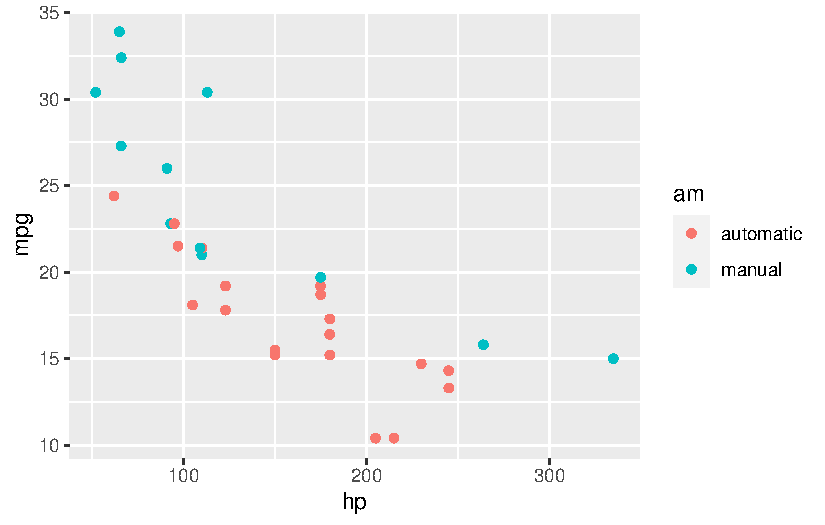
\includegraphics{cv_files/figure-pdf/fig-two-together-1.pdf}

}

\end{figure}

\begin{figure}[H]

\sidecaption{\label{fig-two-together-2}Two plots in one figure
environment.}

{\centering 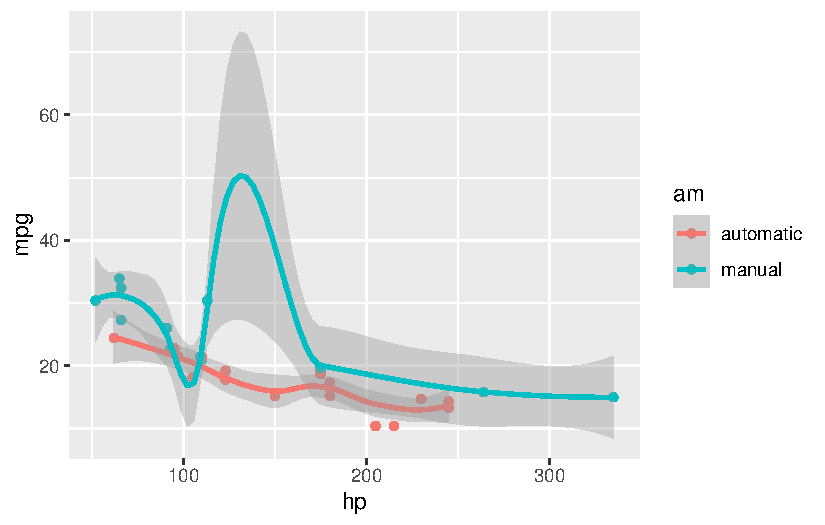
\includegraphics{cv_files/figure-pdf/fig-two-together-2.pdf}

}

\end{figure}

Then two plots in separate figure environments (the code is identical to
the previous code chunk, but the chunk option is the default
\texttt{fig.show\ =\ \textquotesingle{}asis\textquotesingle{}} now):

\begin{Shaded}
\begin{Highlighting}[]
\NormalTok{p }\OtherTok{\textless{}{-}} \FunctionTok{ggplot}\NormalTok{(mtcars2, }\FunctionTok{aes}\NormalTok{(hp, mpg, }\AttributeTok{color =}\NormalTok{ am)) }\SpecialCharTok{+}
  \FunctionTok{geom\_point}\NormalTok{()}
\NormalTok{p}
\NormalTok{p }\SpecialCharTok{+} \FunctionTok{geom\_smooth}\NormalTok{()}
\end{Highlighting}
\end{Shaded}

\begin{figure}[H]

\sidecaption{\label{fig-two-separate-1}Two plots in separate figure
environments (the first plot).}

{\centering 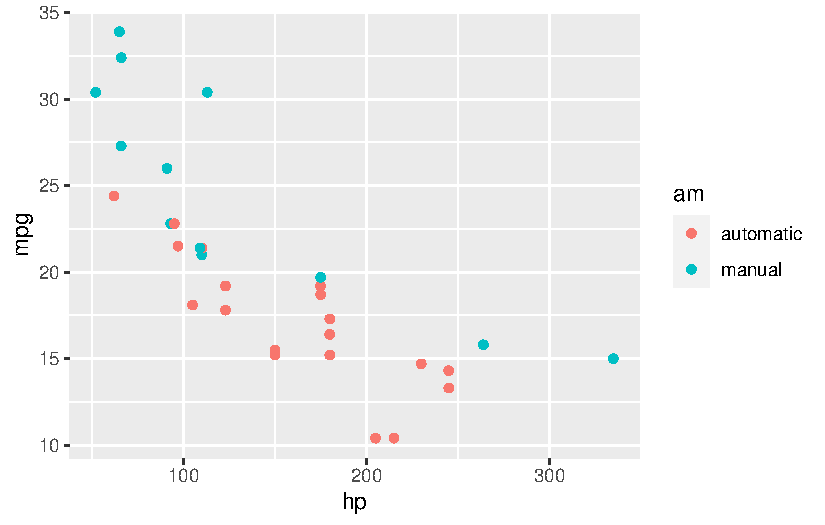
\includegraphics{cv_files/figure-pdf/fig-two-separate-1.pdf}

}

\end{figure}

\begin{figure}[H]

\sidecaption{\label{fig-two-separate-2}Two plots in separate figure
environments (the second plot).}

{\centering 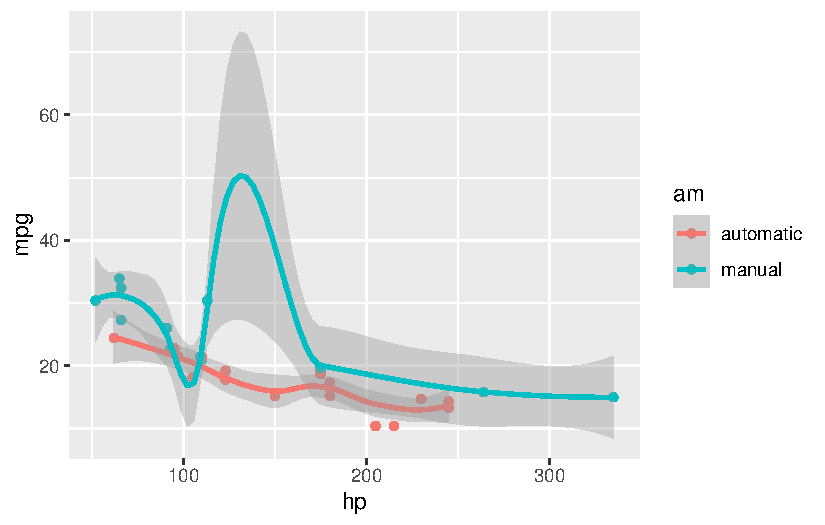
\includegraphics{cv_files/figure-pdf/fig-two-separate-2.pdf}

}

\end{figure}

You may have noticed that the two figures have different captions, and
that is because we used a character vector of length 2 for the chunk
option \texttt{fig.cap} (something like
\texttt{fig.cap\ =\ c(\textquotesingle{}first\ plot\textquotesingle{},\ \textquotesingle{}second\ plot\textquotesingle{})}).

Next we show multiple plots in margin figures. Similarly, two plots in
the same figure environment in the margin:

\begin{Shaded}
\begin{Highlighting}[]
\NormalTok{p}
\NormalTok{p }\SpecialCharTok{+} \FunctionTok{geom\_smooth}\NormalTok{(}\AttributeTok{method =} \StringTok{\textquotesingle{}lm\textquotesingle{}}\NormalTok{)}
\end{Highlighting}
\end{Shaded}

\begin{marginfigure}

{\centering 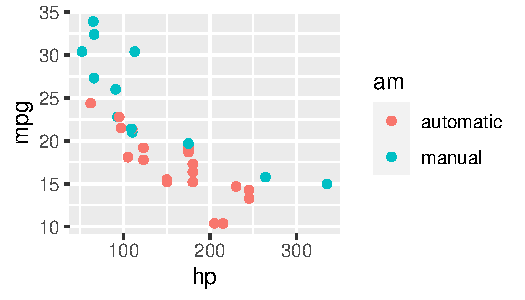
\includegraphics{cv_files/figure-pdf/fig-margin-together-1.pdf}

}

\caption{\label{fig-margin-together-1}Two plots in one figure
environment in the margin.}

\end{marginfigure}

\begin{marginfigure}

{\centering 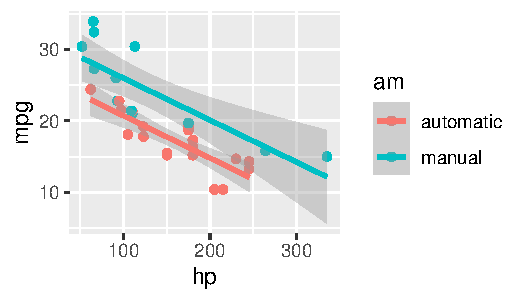
\includegraphics{cv_files/figure-pdf/fig-margin-together-2.pdf}

}

\caption{\label{fig-margin-together-2}Two plots in one figure
environment in the margin.}

\end{marginfigure}

Then two plots from the same code chunk placed in different figure
environments:

\begin{longtable}[]{@{}rrrr@{}}
\toprule()
Sepal.Length & Sepal.Width & Petal.Length & Petal.Width \\
\midrule()
\endhead
5.1 & 3.5 & 1.4 & 0.2 \\
4.9 & 3.0 & 1.4 & 0.2 \\
4.7 & 3.2 & 1.3 & 0.2 \\
4.6 & 3.1 & 1.5 & 0.2 \\
5.0 & 3.6 & 1.4 & 0.2 \\
5.4 & 3.9 & 1.7 & 0.4 \\
4.6 & 3.4 & 1.4 & 0.3 \\
5.0 & 3.4 & 1.5 & 0.2 \\
4.4 & 2.9 & 1.4 & 0.2 \\
4.9 & 3.1 & 1.5 & 0.1 \\
5.4 & 3.7 & 1.5 & 0.2 \\
4.8 & 3.4 & 1.6 & 0.2 \\
4.8 & 3.0 & 1.4 & 0.1 \\
4.3 & 3.0 & 1.1 & 0.1 \\
5.8 & 4.0 & 1.2 & 0.2 \\
\bottomrule()
\end{longtable}

\begin{marginfigure}

{\centering 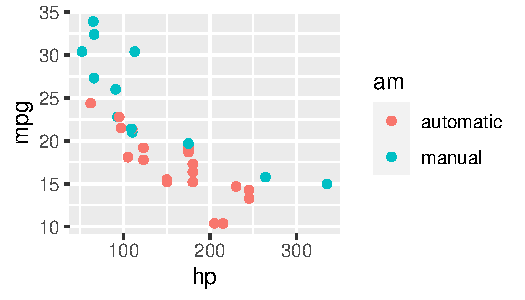
\includegraphics{cv_files/figure-pdf/fig-margin-separate-a-1.pdf}

}

\caption{\label{fig-margin-separate-a-1}Two plots in separate figure
environments in the margin (the first plot)}

\end{marginfigure}

\begin{marginfigure}

{\centering 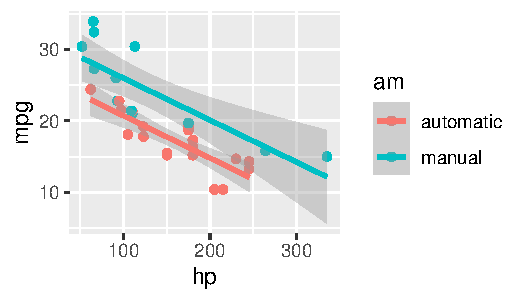
\includegraphics{cv_files/figure-pdf/fig-margin-separate-a-2.pdf}

}

\caption{\label{fig-margin-separate-a-2}Two plots in separate figure
environments in the margin (the first plot)}

\end{marginfigure}

\begin{longtable}[]{@{}rrrr@{}}
\toprule()
Sepal.Length & Sepal.Width & Petal.Length & Petal.Width \\
\midrule()
\endhead
5.1 & 3.5 & 1.4 & 0.2 \\
4.9 & 3.0 & 1.4 & 0.2 \\
4.7 & 3.2 & 1.3 & 0.2 \\
4.6 & 3.1 & 1.5 & 0.2 \\
5.0 & 3.6 & 1.4 & 0.2 \\
5.4 & 3.9 & 1.7 & 0.4 \\
4.6 & 3.4 & 1.4 & 0.3 \\
5.0 & 3.4 & 1.5 & 0.2 \\
4.4 & 2.9 & 1.4 & 0.2 \\
4.9 & 3.1 & 1.5 & 0.1 \\
5.4 & 3.7 & 1.5 & 0.2 \\
4.8 & 3.4 & 1.6 & 0.2 \\
\bottomrule()
\end{longtable}

We blended some tables in the above code chunk only as
\emph{placeholders} to make sure there is enough vertical space among
the margin figures, otherwise they will be stacked tightly together. For
a practical document, you should not insert too many margin figures
consecutively and make the margin crowded.

You do not have to assign captions to figures. We show three figures
with no captions below in the margin, in the main column, and in full
width, respectively.

\begin{Shaded}
\begin{Highlighting}[]
\CommentTok{\# a boxplot of weight vs transmission; this figure}
\CommentTok{\# will be placed in the margin}
\FunctionTok{ggplot}\NormalTok{(mtcars2, }\FunctionTok{aes}\NormalTok{(am, wt)) }\SpecialCharTok{+} \FunctionTok{geom\_boxplot}\NormalTok{() }\SpecialCharTok{+}
  \FunctionTok{coord\_flip}\NormalTok{()}
\end{Highlighting}
\end{Shaded}

\begin{marginfigure}

{\centering 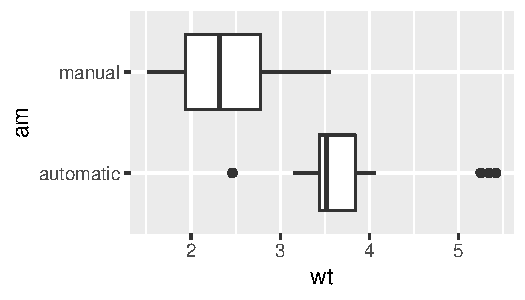
\includegraphics{cv_files/figure-pdf/unnamed-chunk-11-1.pdf}

}

\end{marginfigure}

\begin{Shaded}
\begin{Highlighting}[]
\CommentTok{\# a figure in the main column}
\NormalTok{p }\OtherTok{\textless{}{-}} \FunctionTok{ggplot}\NormalTok{(mtcars, }\FunctionTok{aes}\NormalTok{(wt, hp)) }\SpecialCharTok{+} \FunctionTok{geom\_point}\NormalTok{()}
\NormalTok{p}
\end{Highlighting}
\end{Shaded}

\begin{figure}[H]

{\centering 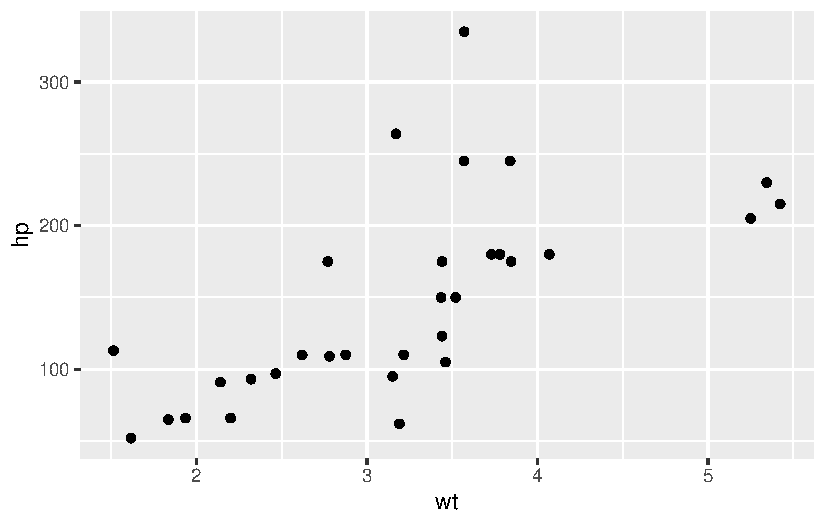
\includegraphics{cv_files/figure-pdf/unnamed-chunk-12-1.pdf}

}

\end{figure}

\begin{Shaded}
\begin{Highlighting}[]
\CommentTok{\# a fullwidth figure}
\NormalTok{p }\SpecialCharTok{+} \FunctionTok{geom\_smooth}\NormalTok{(}\AttributeTok{method =} \StringTok{\textquotesingle{}lm\textquotesingle{}}\NormalTok{) }\SpecialCharTok{+} \FunctionTok{facet\_grid}\NormalTok{(}\SpecialCharTok{\textasciitilde{}}\NormalTok{ gear)}
\end{Highlighting}
\end{Shaded}

\begin{figure*}[H]

{\centering 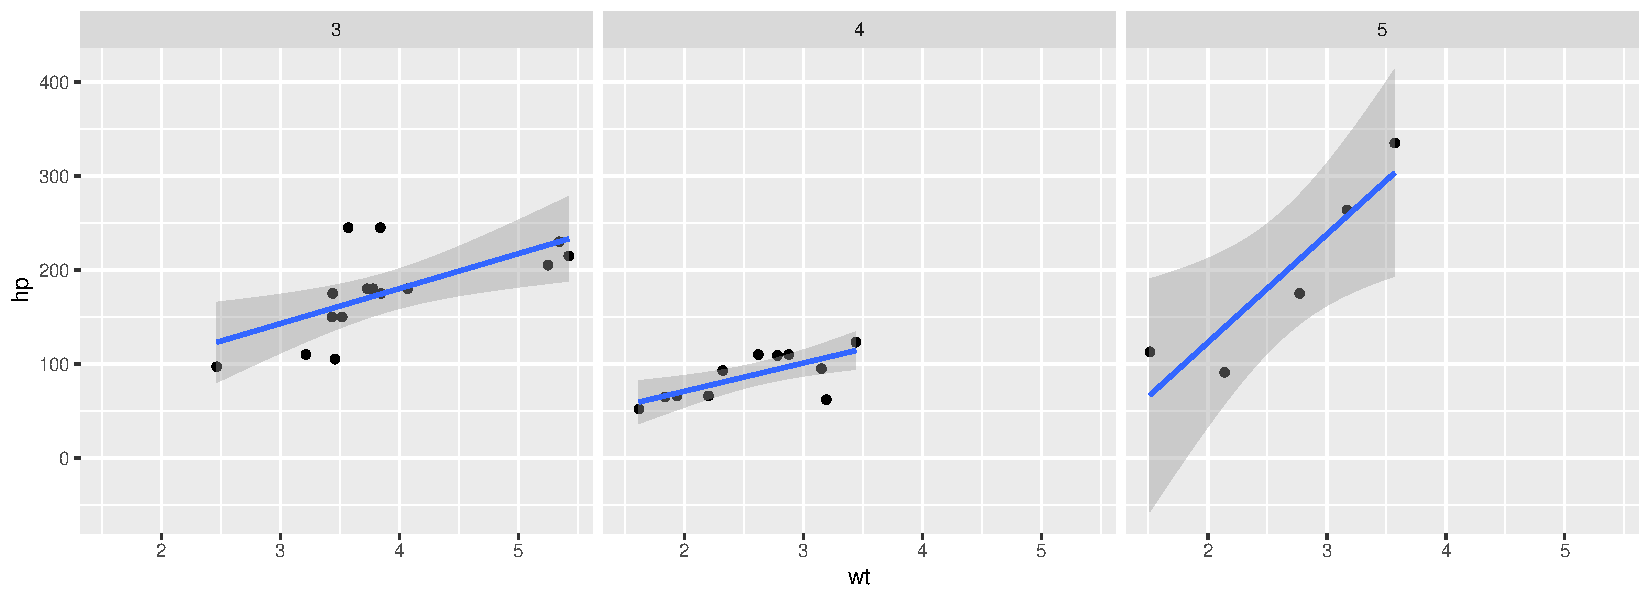
\includegraphics{cv_files/figure-pdf/unnamed-chunk-13-1.pdf}

}

\end{figure*}

\hypertarget{some-notes-on-page-layout}{%
\section{Some Notes on Page Layout}\label{some-notes-on-page-layout}}

To see the Quarto markdown source of this example document, you may
follow
\href{https://raw.githubusercontent.com/quarto-dev/quarto-gallery/main/page-layout/tufte.qmd}{this
link to Github}.



\end{document}
